\documentclass[14pt]{extarticle}

\usepackage{fontspec}
\usepackage{polyglossia}
\usepackage[a4paper, % Согласно требованиям к ВКР
  lmargin=30mm, rmargin=15mm, tmargin=20mm, bmargin=20mm]{geometry}
\usepackage{multirow}


\setdefaultlanguage{russian}
\setotherlanguage{english}

\usepackage{listings}
\usepackage{color}

\definecolor{dkgreen}{rgb}{0,0.6,0}
\definecolor{gray}{rgb}{0.5,0.5,0.5}
\definecolor{mauve}{rgb}{0.58,0,0.82}

\lstset{frame=tb,
  language=Java,
  aboveskip=3mm,
  belowskip=3mm,
  showstringspaces=false,
  columns=flexible,
  basicstyle={\small\ttfamily},
  numbers=none,
  numberstyle=\tiny\color{gray},
  keywordstyle=\color{blue},
  commentstyle=\color{dkgreen},
  stringstyle=\color{mauve},
  breaklines=true,
  breakatwhitespace=true,
  tabsize=3
}

% Согласно требованиям к ВКР
\defaultfontfeatures{Ligatures=TeX}

\setmainfont{Times New Roman}
\setmonofont{Courier New}
\setsansfont{Arial}

\newfontfamily\cyrillicfont{Times New Roman}
\newfontfamily\cyrillicfontsf{Arial}
\newfontfamily\cyrillicfonttt{Courier New}

\newfontfamily\englishfont{Times New Roman}
\newfontfamily\englishfontsf{Arial}
\newfontfamily\englishfonttt{Courier New}

\linespread{1.5}

\usepackage[backend=biber,
  bibencoding=utf8,
  sorting=none,
  style=gost-numeric,
  language=autobib,
  autolang=other,
  clearlang=true,
  defernumbers=true,
  sortcites=true,
  doi=true,
  isbn=true,
  ]{biblatex}

\bibliography{bibliography.bib}

\usepackage[dvipsnames]{xcolor}
\usepackage[hidelinks,colorlinks=true,citecolor=BurntOrange,urlcolor=Blue]{hyperref}
\renewcommand{\UrlFont}{\small\rmfamily\tt}


\renewcommand\thesection{\arabic{section}}

\usepackage{amsfonts}

\usepackage{tikz}
\usepackage{pgfplots}
\usepackage{wrapfig}

\usepackage{graphicx}
\graphicspath{ {./images/} }


\renewcommand*{\maketitle}{
\begin{titlepage}
  \begin{center}
    \linespread{1}
    \small
    Федеральное государственное автономное образовательное учреждение\break высшего образования\par
    <<Московский физико-технический институт \break (национальный исследовательский университет)>>\par
    Физтех-школа Прикладной Математики и Информатики\par
    Кафедра корпоративных информационных систем\par
  \end{center}
%
  {
    \small
    {\bf Направление подготовки / специальность}: 01.03.02 Прикладная математика и информатика\newline
    {\bf Направленность (профиль) подготовки}: Прикладная математика и компьютерные науки
  }
%
  {
    \topskip0pt
    \vspace*{\fill}
    \begin{center}
      {\bf\Large РАЗРАБОТКА ПОДСИСТЕМЫ, ОТВЕЧАЮЩЕЙ ЗА ИЗМЕНЕНИЯ КОНФИГУРАЦИИ СЕРВИСОВ ДЛЯ SERVICE MESH
      \break }\par
      (бакалаврская работа)
    \end{center}
    \vspace*{\fill}
  }
%
  \hfill
  \begin{minipage}[t]{8cm}
    {\bf Студент: \newline}
    Сагитов Искандер Рустамович\newline
    \vspace{-3mm}
    \rule{8cm}{0.15mm}
    \centerline{\scriptsize\it (подпись студента)}\newline
%
    {\bf Научный руководитель: \newline}
    Шмарион Максим Юрьевич\newline
    \vspace{-3mm}
    \rule{8cm}{0.15mm}
    \centerline{\scriptsize\it (подпись научного руководителя)}\newline
%
    {\bf Научный консультант: \newline}
    Буланкин Данил Андреевич \newline
    \vspace{-3mm}
    \rule{8cm}{0.15mm}
    \centerline{\scriptsize\it (подпись научного консультанта)}
%
  \end{minipage}

    \vspace*{\fill}
    \begin{center}
      Москва 2022
    \end{center}
\end{titlepage}
}


\begin{document}
\maketitle

\newpage
\setcounter{page}{2}

\vspace*{\fill}
\begin{abstract}

Данная работа посвящена иследованию существующих решений Service Mesh и проектированию архитектуры для собственной реализации данного приложения. Также в работе реализуется часть спроектированного Service Mesh такие как набора инструментов для упрощенного создания прокси для управления всем траффиком в сети, где будет работать Service Mesh и подсистема Controller, отвечающая за доставление необходимых настроек до этих прокси.\end{abstract}
\vspace*{\fill}

\newpage
\tableofcontents
\newpage


\section{Введение}
\label{sec:intro}
\subsection{Проблемы микросервисной архитектуры}
%Исторически, приложения проектировались в соответствии с монолитной архитектурой, но постепенно стали появляться приложения реализованные в соответствии с  микросервисной архитектурой. Обычно этот переход сопровождает вынос части логики из монолита в межсервисное взаимодействие. В связи с этим усложнялся програмный код - в монолитной архитектуре разные части приложения могли просто вызывать функции из других частей, но при переходе на новую архитектуру так делать уже нельзя, ведь эти разные компоненты могут даже находиться на разных физических хостах и приходится уже общаться через сеть, что вызывает дополнительные нагрузки на разработку и эффективность работы программы.
Компании вс ечаще задумываются над переносом своего монолитного приложения на микросервисную архитектуру. Также многие компании используют облака для развертывания своих микросервисов. Как известно, монолитные приложения сложны при програмировании и у них длинный релизный цикл.

В то время как микросервисная архитектура способствует ускорению релизного цикла и ускорению разработки, оно также добавляет некие новые сложности, например такие, как описанные ниже.
\begin{itemize}
	\item Безопасность -- в отличие от монолитного приложения, где одни функции просто вызывают другие, в микросервисной архитектуре это обычно трансформируется в запросы по сети из одного сервиса в другой с необходимостью отслеживать всю эту коммуникацию.
	\item Отказоустойчивость -- значительно увеличивается граф зависимостей между сервисами, что ведет к замедлению работы программы из-за большого количества последовательных запросов по сети и также повышает вероятность каскадного отказа сервисов из-за отказа всего лишь одного.
	\item Правила межсервисного взаимодействия -- некоторые сервисы могут становиться узкими местами при выполнениях функций других сервисов. Необходимо настраивать квоты и определять политики, котороые описывают какие сервисы к каким могут совершать вызовы и как много таких вызовов может совершаться.
	\item Наблюдаемость -- по сравнению с монолитными приложениями, где достаточно файлов лога, в микросервисной архитектуре один полноценный запрос может проходить через несколько приложений. Получается, что ошибка может возникнуть в любом месте этой цепочки и разработчикам необходимо не только хранить файлы лога, но и иметь возможность следить за сетевыми показателями сервисов, процессом прохождения через цепочку сервисов отдельного запроса и за топологией всего кластера.
\end{itemize}

\subsection{Service Mesh}
Service Mesh -- отдельный уровень в микросервисной архитектуре, который абстрагирует в себе межсетевое взаимодействие отдельных сервисов и позволяет единообразным образом, независимо от кода отдельных приложений, решать следующие проблемы:

\begin{itemize}
	\item Обеспечение безопасности -- традиционная сетевая безопасность основана на обеспечении надежного периметра для предотвращения доступа злоумышленника внутрь. Service Mesh же, в свою очередь, предоставляет идентификатор для каждого сервиса и уже по этим идентификаторам происходит аутентификация и авторизация, обеспечивается контроль того,  как различные сервисы могут общаться между собой. Также Service Mesh позволяет разработчикам использовать различные протоколы, например mTLS для обеспечения зашифрованного трафика между сервисами и предотвращения атак men-in-the-middle.
	\item Наблюдаемость -- из-за особенностей реализации Service Mesh, весь сетевой трафик внутри сети протекает через него. Далее, Service Mesh генерирует необходимые типы телеметрии: метрики, трейсы, логи доступов и складывает в хранилище.
	\item Балансировка нагрузки -- обычно у каждого сервиса запущено несколько инстансов и общая нагрузка распределяется между ними. В качестве способа балансирования часто используют алгоритм round-robin(равномерное распределение запросов к каждому инстансу) или взвешенный round-robin(то же самое, что и round-robin, но у каждого инстанса есть свой вес) или же случайный что не учитывает, например, того, что разные запросы могут быть разной сложности. Service Mesh же, имея у себя все необходимые метрики, позволяет использовать более умные алгоритмы балансировки нагрузки.
	\item Поиск сервисов -- часто у сервисов меняется количество инстансов или сами инстансы меняют физические хосты. Service Mesh может обрабатывать эти ситуации и самостоятельно перенаправлять запросы к живым, в текущий момент, инстансам используя определенное ранее правило балансировки.
\end{itemize}

Обычно архитектура Service Mesh делится на 2 концептуальные части:
\begin{itemize}
	\item Data plane -- обычно это набор проксей, которые перехватывают весь входящий и исходящий трафик конкретного сервиса и перенаправляет его в соответствии со своей конфигурацией. Также эти прокси собирают телеметрию и отправляют ее в Service Mesh.
	\item Control plane -- набор приложений в Service Mesh, которые отслеживают состояния всех сервисов и в соответствии с этим переконфигурируют прокси.
\end{itemize}

\subsection{Существующие решения}

Рассмотрим самые популярные реализации Service Mesh.

\begin{itemize}
	\item Istio -- open source решение от Google, которое в качестве прокси использует Envoy. Istio имеет широкие возможности конфигурации, но потребляет достаточно большое количество ресурсов. Изначально Istio спроектировано для работы с кластером Kubernetes, но его также можно использовать и с пользовательской системой развертывания. В итоге, если суметь сконфигурировать Istio, то получиться достаточно универсальный инструмент, который решает перечисленные выше проблемы, но тут ощущается недостаток документации и статей о том, как сделать что-то.
	\item Linkerd -- open source решение, которое в качестве Data Plane использует собственную легковесную прокси, из-за чего накладные расходы от Service Mesh в разы меньше. Linkerd предоставляет меньше возможностей конфигурации, что делает эту самую конфигурацию более простой.
\end{itemize}

Получается, что Linkerd подходит для тех, кому нужен просто быстрый Service mesh который практически не надо конфигурировать, в случае же когда от Service Mesh требуются специфические настройки, то следует использовать Istio.

Мы же, в свою очередь, хотим настроить Service Mesh для 1С Облака, в котором имеется своя собственная система развертывания и где не используется Kubernetes. Из-за этого Linkerd нам точно не подходит, потому что он не используется вне Kubernetes. Istio нам также не подходит так как, хоть его и можно использовать вне Kubernetes, но для этого не хватает документации.

В итоге мы пришли к тому, что нам необходимо разработать собственное решение данной задачи. Мы остановились на том, что на данный момент из всей функциональности Service Mesh нам необходимо реализовать только следующий набор:
\begin{itemize}
	\item Мониторинг
	\item Балансировка
	\item Автоматическое перенаправление запросов 
\end{itemize}

\subsection{Цель и задачи}

Целью работы является реализации компоненты Service Mesh, которая отвечает за переконфигурирование sidecar-proxy. В качестве прокси мы решили использовать Envoy так как он позволяет себя динамически переконфигурировать.
\begin{itemize}
	\item исследовать текущие решения и спроектировать архитектуру Service Mesh
	\item определить, какую прокси следует использовать в Data Plane
	\item реализовать набор инструментов для упрощения создания стартовых конфигураций прокси
	\item реализовать приложение Controller, которое ответственно за доставку новых конфигураций для этих прокси
	 \item протестировать приложение Controller и инструменты для изначального начального запуска прокси
\end{itemize}

В результате работы были получены следующие результаты:
\begin{itemize}
    \item создана архитектура Service Mesh
	\item выбран Envoy в качестве прокси для Data Plane
	\item написан bash-скрипт для создания начальной конфигурации Envoy
	\item реализовано приложение Controller
	\item реализовано отдельное приложение для тестирования приложения Controller и bash-скрипта
\end{itemize}
%(https://linkerd.io/2021/05/27/linkerd-vs-istio-benchmarks/?_gl=1*40ac7o*_ga*MTgzNzM2NTQ2My4xNjUyMjU3NDE3*_ga_TV358ZPK6D*MTY1MjQ0ODIyOS4zLjEuMTY1MjQ0ODIzMC4w#_ga=2.221305884.50908095.1652424877-1837365463.1652257417)


\section{Разработанное решение}

\subsection{Архитектура Service Mesh}
Также, как и в большинстве реализаций, мы разделили разделили все компоненты на 2 концептуальные части:
\begin{itemize}
	\item Data Plane -- для каждого сервиса, у которого есть множество инстансов, будет стоять одна прокси на вход, то есть все поступающие запросы будут проходить через эту прокси и она будет решать, в какой инстанс его направить. Также будет одна прокси на выход, то есть если инстансу необходимо воспользоваться другим сервисом, то он направляет запрос в эту прокси и уже она, зная, где находится прокси на вход у этого сервиса, перенаправляет запрос туда.
	\item Control Plane -- мы решили разделить эту часть на несколько приложений:
\begin{enumerate}
	\item Service Discovery -- сервис, который знает, на каком хосте и на каком порту находится каждый инстанс каждого приложения и который также умеет получать запросы о том, что какой-то инстанс поднялся, или наоборот - пропал.
	\item Controller -- сервис, который от Service Discovery получает более конкретный запрос, что в связи с изменением конфигурации кластера следуют переконфигурировать следующие инстансы Envoy и то, как именно их стоит переконфигурировать
	\item Monitoring service -- сервис для отслеживания состояния Envoy
	\item Balancing service -- сервис для настройки балансировки между инстансами отдельного сервиса
\end{enumerate}
\end{itemize}

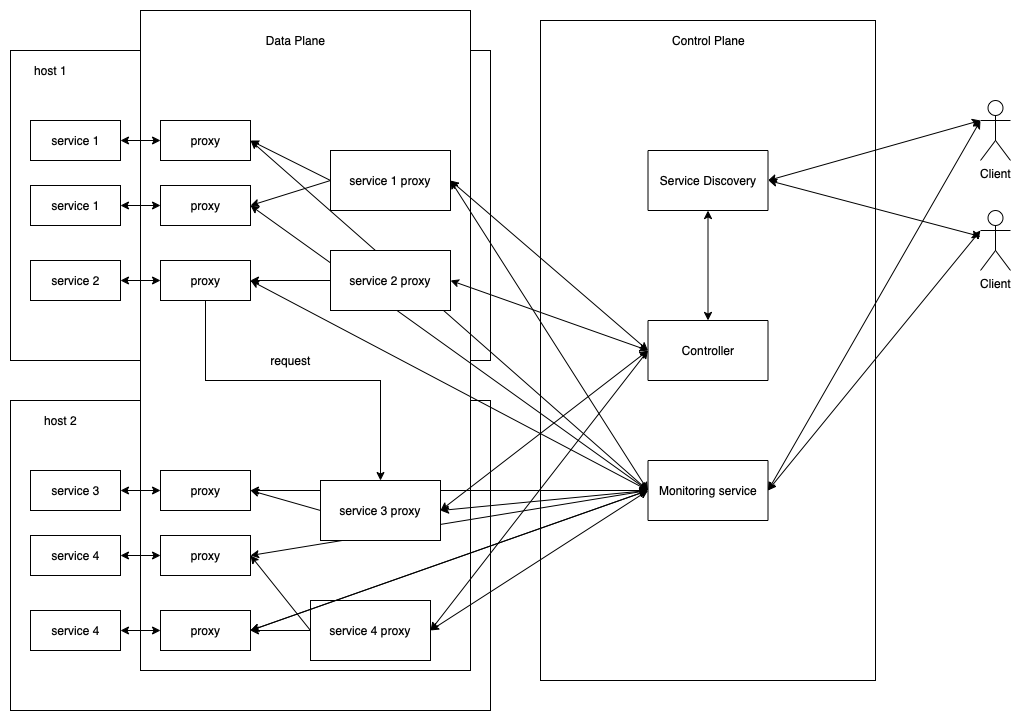
\includegraphics[width=\textwidth]{ServiceMeshArchitecture.drawio.png}

Как видно на схеме, клиенты обращаются к Service Discovery с верхнеуровневыми запросами, что у какого-то сервиса надо добавить, или наоборот, убрать инстанс. Далее, Service Discovery обрабатывает этот запрос и в процессе создает пачку запросов к Controller, что для некоторых proxy надо поменять конфигурацию, например, в случае удаления инстанса сначала надо убрать из под нагрузки, а потом выключать, а в случае добавления сервиса следует делать наоборот - сначала поднять инстанс и уже потом переконфигурировать прокси, чтобы на этот инстанс тоже шли запросы.

Сам же трафик в сети ходит следующим образом:
\begin{enumerate}
	\item Выходящие запросы из инстансов сервисов всегда направляются в прокси этих инстансов.
	\item Эти прокси перенаправляют запросы к нужным прокси сервисов.
	\item Прокси сервиса перенаправляет запрос в прокси нужного инстанса.
	\item Прокси инстанса перенаправляет запрос к инстансу.
\end{enumerate}

Также пользователь может получать различные метрики о состоянии кластера. Для этого ему достаточно делать запросы к компоненте Monitoring Service, которая, в свою очередь опрашивает все прокси связанные с нужным сервисом. А прокси имеют все необходимые метрики так как через них проходят все запросы.
\subsection{Выбор proxy для Data Plane}

Изначально мы рассматривали 3 варианта:

%https://blog.getambassador.io/envoy-vs-nginx-vs-haproxy-why-the-open-source-ambassador-api-gateway-chose-envoy-23826aed79ef
\begin{itemize}
	\item Nginx \cite{nginx} -- высокопроизводительный веб-сервер, поддерживающий hot reload(применение изменений без перезагрузки сервера), но его также можно использовать как reverse-proxy, в каччестве кеша или балансировщика нагрузки. Nginx использует асинхронную событийно-ориентированную модельобработки запросов, то есть на каждый запрос не создается отдельный поток выполнения, а все запросы обрабатываются в одном потоке, но не блокирую друг друга. К сожалению, open-source версия nginx имеет ряд ограничений, например hot reload не может выполняться при большой нагрузке и теряет часть пакетов и также отсутствует health checking(периодические проверки инстансов на то, что они могут принимать запросы). 
%https://engineeringblog.yelp.com/2015/04/true-zero-downtime-haproxy-reloads.html
	\item HAProxy(High Availability Proxy) \cite{HAProxy} -- популярное программное обеспечение с открытым исходным кодом для балансировки нагрузки HTTP/TCP траффика или выступающее в качестве прокси-сервера. HAProxy также как и nginx использует один процесс и событийно-ориентированную модель обработки запросов, что позволяет при использовании достаточно маалого объема памяти обрабатывать одновременно множество запросов.
	\item Envoy \cite{Envoy} -- самый молодой(появился в 2016 году) прокси из этих трех, но который уже используется в таких компаниях как Lyft, Google, Apple и других. Envoy изначально был спроектирован для работы с микросервисами так как имеет такие функции как hot reload, наблюдаемость, отказоустойчивость и продвинутая балансировка нагрузки. Envoy также может использоваться в ситуации частых изменений конфигураций приложений так как предоставляет не только статическую конфигурацию, но и динамическую, например, с помощью gRPC/protobuf.
\end{itemize}

В итоге мы решили остановиться на Envoy из-за того, что он поддерживает динамическую переконфигурацию то есть можно поменять конфигурацию без перезагрузки.

Envoy внутри себя определяет несколько ресурсов конфигурации, но нам интересны только следующие:
\begin{enumerate}
	\item listener -- адрес и порт, на которых слушает Envoy. С помощью listener'ов Envoy получает соединения и запросы. Envoy может иметь как и более одного listener'a, также как и один listener может слушать более чем на одном IP-адресе.
	\item route -- наборы правил, связанные с listener'ами, которые сопоставляют виртуальные хосты с кластерами. В этих правилах можно опираться на метаданные запроса, такие как заголовки или URI и в зависимости от этого определять, на какой кластер его следует направить.
	\item cluster -- набор вышестоящих хостов, которые обрабатывают получаемые запросы. Также cluster'ы являются теми ресурсами, в которых можно прописывать правила балансировки, таймауты подключения и автоматические выключения.
\end{enumerate}
Envoy поддерживает статическую конфигурацию, то есть когда изначально в .yaml файле прописаны все настройки, и динамическую, то есть когда в .yaml файле прописан способ получения конфигурации.

В свою очередь динамическая конфигурация бывает трех типов:
\begin{enumerate}
	\item Подписка на файл -- самый простой способ получения динамической конфигурации это поместить ее по известному локальному пути и прописать этот путь в конфигурацонный файл. В таком случае Envoy, в зависимости от операционной системы, использует inotify или kqueue для отслеживания изменений в файле. Также в этом случае нет механизма решать конфликты при ошибках обновления конфигурации, поэтому при возникновении ошибок при. обновлении Envoy будет просто откатываться на предыдущую версию.
	\item gRPC stream -- примерно как предыдущий вариант, но вместо отправления запросов Management Server'у поддерживается gRpc stream с ним.
	\item REST -- также возможен способ получения обновлений через периодические запросы к Management Server'у с использованием протокола REST, но в этом случае постоянное соединение с сервером не поддерживается. Ожидается, что в любой момент времени существует не более одного запроса к Management Server'у.
\end{enumerate}

В нашей ситуации конфигурация Envoy, который выступает в роли sidecar'a у инстанса сервиса будет состоять из следующих частей:
\begin{itemize}
	\item Для каждого другого сервиса, который используется этим инстансом мы добавляем пару listener -- cluster, чтобы перенаправлять запрос.
	\item Одна пара listener -- cluster для слушания и перенаправления запросов, которые должны передаваться конкретно этому инстансу.
	\item Также требуется добавить по одному route для каждой пары listener -- cluster, описанных выше из-за особенностей Envoy.
\end{itemize}

Конфигурация Envoy, который выступает в роли прокси для сервиса будет состоять из следующих частей:
\begin{itemize}
	\item Один cluster для настройки правил в каком случае какому инстансу следует перенаправть конкретный запрос.
	\item Один listener для слушания запросов, которые должны передаваться конкретно этому сервису.
	\item Также требуется добавить один route для вышеописанной пары listener -- cluster, из-за особенностей Envoy.
\end{itemize}

Понятно, что статическая конфигурация и динамическая с подпиской на файл нас не устраивали. Разницы между оставшимися вариантами практически нет, но вариант с использованием REST'a больше не поддерживается в третьей версии Envoy'a, так что я решил использовать динамическую конфигурацию с использованием gRPC для получения новой версии.

\subsection{Конфигурация Envoy}
На более глубоком уровне разделяется 4 варианта транспортного протокола, которые складываются из двух измерений, в каждом из которых можно выбрать один из двух вариантов.

Первое измерение это State of the World (SotW) vs Incremental:
\begin{enumerate}
	\item State of the World -- Envoy определяет ресурсы, на которые он подписывается и каждый раз при запросе новой конфигурации требуется предоставить все ресурсы.
	\item Incremental -- Envoy также определяет ресурсы, на которые он подписывается, но при получении новой конфигурации следует предоставить только те ресурсы, которые поменялись.
\end{enumerate}
Ключевая разница между ними заключается в том, что если, например, Envoy подписался на изменения 100 ресурсов и изменился ровно 1 ресурс, то в первом случае требуется выслать конфигурацию со всеми 100 ресурсами, а во втором только изменившийся ресурс. К счастью, в нашем случае разница не так велика. 

Заметим, что прокси которые связаны с сервисом имеют только 3 ресурса, так что тут разницы примерно нет, так как это маленькая конфигурация.

А в случае же прокси, которые выступают в роли sidecar'ов к инстансам сервисов есть 2 концептуально различающихся варианта, когда меняется конфигурация:
\begin{enumerate}
	\item Меняется состояние инстанса -- например, он начинает пользоваться новым сервисом или слушать на другом адресе, но тогда вместе с переконфигурацией прокси также происходит передеплой самого инстанса. Но тогда самая дорогая часть всепого передеплоя это как раз само разворачивание инстанса сервиса, ну и тогда мы можем позволить себе полностью переконфигурировать прокси.
	\item Меняется адрес прокси другого сервиса, адрес которого присутствует в одном из cluster'ов этого прокси -- мы считаем, что наши прокси "прибиты гвоздями" и их адреса практически не меняются. Поэтому этим случаем тоже можно пренебречь.
\end{enumerate}

Получается, что лучшее решение это использовать Incremental подход но в конкретно нашей задаче при использовании State of the World проигрыш в производительности практически незаметен, поэтому я решил остановиться на последнем ради упрощения реализации и поддержки в будущем.

Другим же измерением является выбор между использованием отдельного gRPC-stream'a для каждого типа ресурса или же использовать один gRPC-stream для передачи всех ресурсов. Изначально Envoy поддерживал только первый вариант, то есть использование различных gRPC-stream'ов для разных типов ресурсов, но тогда при неаккуратной отправке ресурсов Envoy мог терять часть трафика, например, из-за следующей проблемы. Представим, что у нас был listener A, который перенаправляет запросы в cluster B. Дальше пришло обновление конфигурации, из-за которого listener A начинает перенаправлять запросы в кластер C, но cluster'a С в конфигурации нет. И получается, что весь этот трафик будет пропадать до тех пор, пока в gRPC-stream'e для cluster'ов не придет cluster C. Выглядит, что не стоит поддерживать несколько gRPC-stream'ов между двумя сервисами, когда можно обойтись одним и также мы не хотим терять трафик из-за таких незначительных проблем , поэтому для решения этих проблем я буду использовать второй вариант -- единый gRPC-stream для всех типов ресурсов и также для решения последней проблемы порядок между ресурсами будет следующим:
\begin{enumerate}
	\item cluster -- сначала отправляем все необходимы кластеры так как они не используют другие типы ресурсов
	\item listener -- в наших конфигурациях listener'ы используют только cluster'ы, поэтому после доставки cluster'ов можно отправить listener'ы. На самом деле listener еще неявно использует route ресурс, раз я всегда обновляю всю конфигурацию, то необходимые route'ы я буду отправлять вместе с listener'ом, для которого они требуются.
\end{enumerate} 

Вышеописанные рассуждения можно проиллюстрировать следующей таблицей, добавив, что я реализую вариант из левого нижнего угла.
\begin{table}[ht]
\small
\centering
\begin{tabular}{ p{30mm} | p{30mm} |  p{30mm} }
                      &  State of the World (SotW) & Инкрементальный подход \\
\hline
Отдельный gRPC-stream для каждого типа ресурса   & Всегда обновляется вся конфигурация и для разных типов ресурсов используются разные gRPC-stream'ы & Обновляются только изменившиеся ресурсы и для разных типов ресурсов используются разные gRPC-stream'ы \\
\hline
Общий gRPC-stream для всех ресурсов                 & Всегда обновляется вся конфигурация и используется единственный gRPC-stream для передачи всех ресурсов & Обновляются только изменившиеся ресурсы и  используются единственный gRPC-stream \\
\end{tabular}
\caption{Варианты транспортного протокола}
\end{table}

\subsection{Изначальная настройка конфигурации Envoy}

Как было описано выше, наша цель заключается в том, что мы хотим динамически подгружать все необходимые ресурсы, но для этого необходимо не только запустить приложение, которое будет поставлять ресурсы, но и сообщить Envoy'у, как он будет себя идентифицировать, в каком формате будут поступать ресурсы, с помощью какого протокола будет происходить общение с сервером и также определить, по какому адресу будет админ панель, которая нужна для Monitoring Service.

Панель администратора нужна для двух вещей. Во первых, она позволяет получать приватную информацию о состоянии инстанса Envoy, и, во вторых, она предоставляет возможность администраторам управлять состоянием инстанса, например выключить его. В данной ситуации конфигурация достаточно проста и просто содержит адрес, на котором Envoy будет слушать запросы к панели администратора.

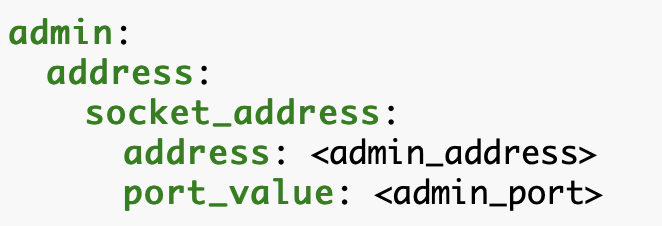
\includegraphics[width=0.5\textwidth]{admin.png}

Management Server может поддерживать gRPC-stream'ы сразу с несколькими инстансами Envoy, поэтому необходим механизм для того, чтобы определять, какому инстансу Envoy какая конфигурация соответствует. Для решения этой задачи в изначальной конфигурации можно определить 2 строковых поля node.cluster и node.cluster. Названия этих полей хорошо сочетаются с выбранной нами архитектурой для Service Mesh так как у нас инстансы Envoy тоже поделены на кластера по принципу один кластер инстансов Envoy для множества инстансов одного сервиса, а внутри кластера они также поделены на sidecar-proxy отдельных инстансов сервиса и на отдельный Envoy-balancer.

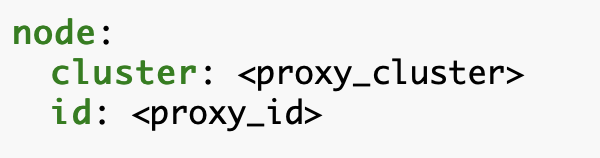
\includegraphics[width=0.5\textwidth]{id.png}

Далее следует определить протокол, по которому будут передаваться ресурсы с Management Server'а. Мы будем пользоваться V3 версией транспортного протокола, так как это самая новая, на данный момент, версия и также будем использовать единый gRPC-stream для получения всех типов ресурсов. Здесь также требуется указать сами настройки общения с Management Server'ом, но пока можно сказать, что это будет ресурс типа cluster с именем xds\_cluster и мы определим его чуть ниже. Также здесь необходимо указать протокол получения ресурсов типов cluster и listener(параметры dynamic\_resources.cds\_config и dynamic\_resources.lds\_config), которые в нашем случае получаются через агрегированный стрим и что будет использоваться V3 версия api.

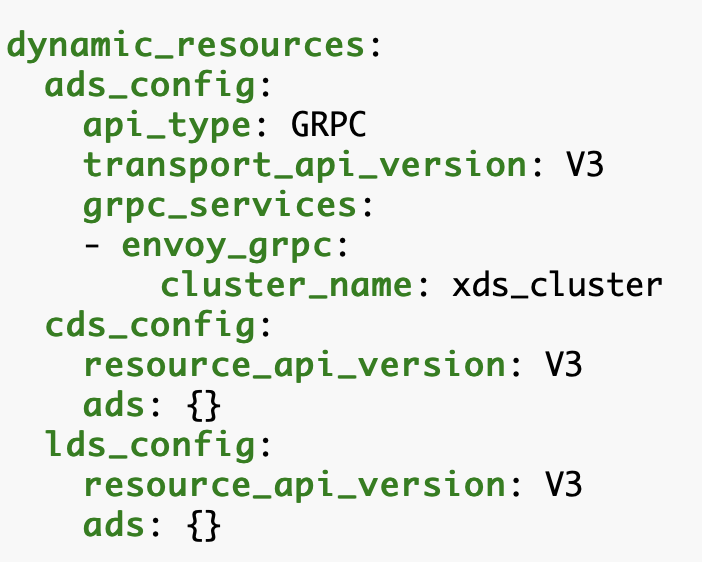
\includegraphics[width=0.5\textwidth]{dynamic.png}

Настройка же ресурса xds\_cluster находится в статической части конфигурации. В ней следует указать адрес Management Server'a, настроить протокол и указать таймауты. В качестве протокола я решил использовать http2, в качестве адреса Management Server'a следует указывать адрес Controller'a, откуда впоследствии будут получаться новые конфигурации. В качестве таймаутов были выбраны дефолтные значения в виде 5 и 30 секунд и при тестировании приложение было решено их оставить.


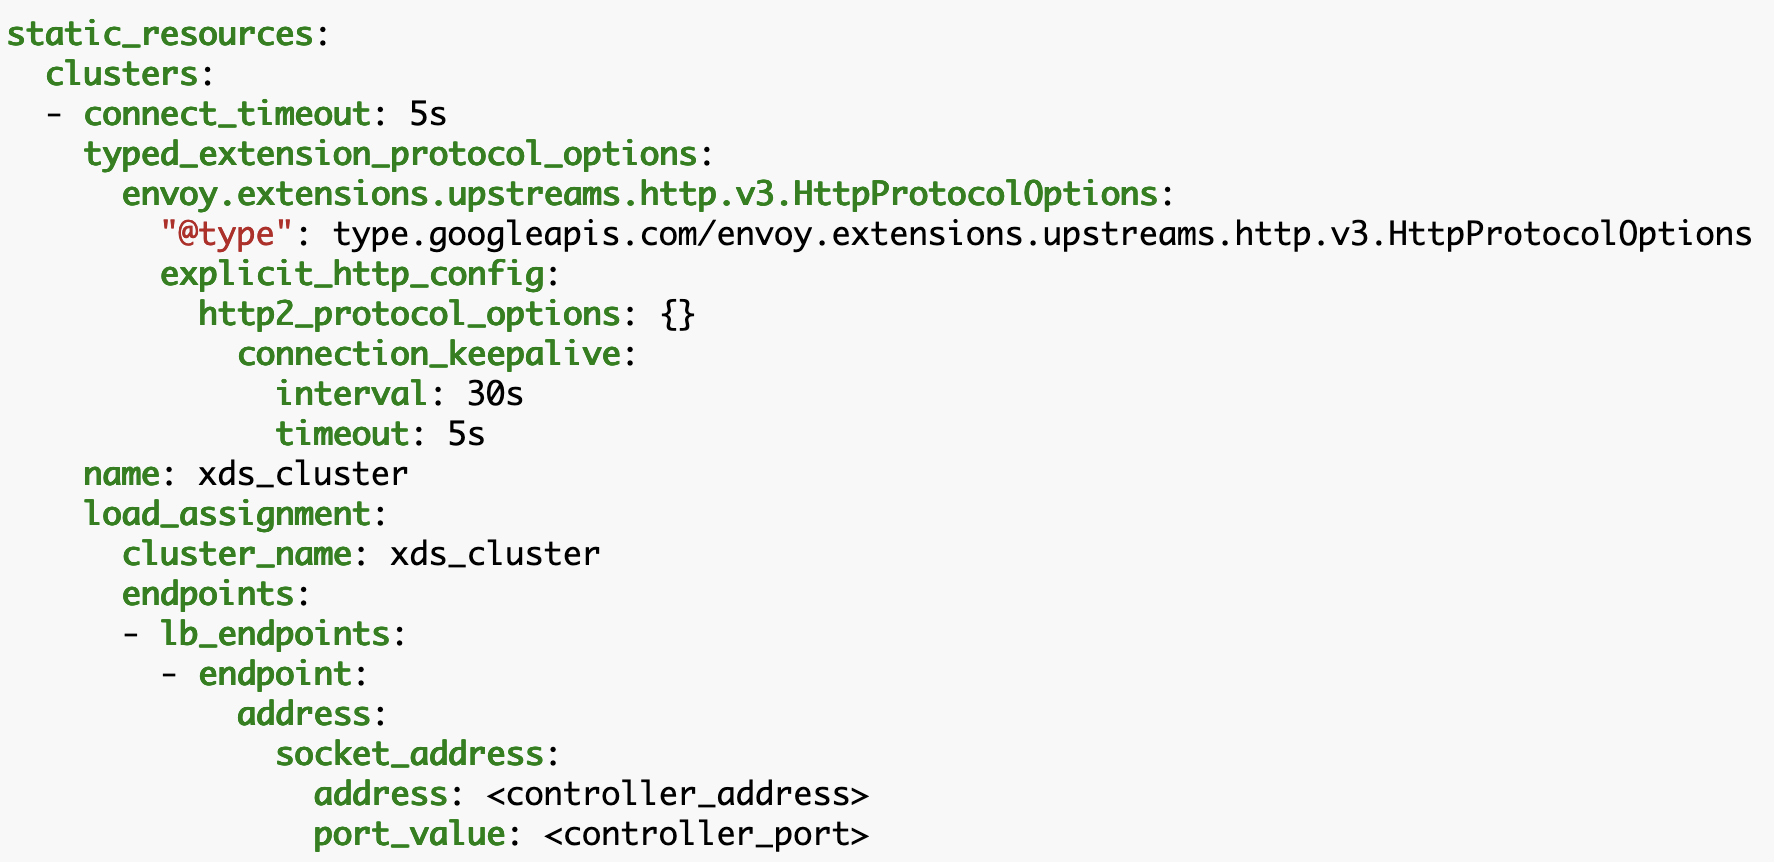
\includegraphics[width=\textwidth]{static.png}

Как мы видим, у нас в системе есть много Envoy-proxy, каждый из которых требует свой изначальный конфигурационный файл. Также можно заметить, что каждый из этих файлов содержит совпадающие части такие как настройка транспортного протокола Envoy, "почти" совпадающие части такие как таймауты, так как дефолтные таймауты будут хороши почти всегда, но в некоторых ситуациях их будет необходимо дополнительно настраивать и части конфигурации, которые из раза в раз будут меняться, например, идентификатор node.cluster и node.id. Поэтому, для упрощения написания конфигурации для Envoy я написал bash-скрипт, который можно найти по адресу \url{https://github.com/iskander232/Controller/blob/master/create_envoy_config.sh} в качестве аргументов принимает опции конфигурации Envoy, такие как:
\begin{itemize}
	\item --cluster-id -- cluster.id
	\item --node-id -- node.id
	\item --controller-port -- порт, через который устанавливается gRPC-stream с Controller'ом
	\item --controller-address -- адрес, через который устанавливается gRPC-stream с Controller'ом
	\item --admin-api-port -- порт панели администратора
	\item --admin-api-address -- адрес панели администратора
\end{itemize}

Скрипт можно запускать следующей командой, после исполнения которой в stdout будет написан корректный файл конфигурации созданный по вышеописанным правилам, который, например, с помощью перенаправления потока можно записать в файл и потом на основе этого конфига запустить Envoy. Также на основе вывода скрипта видно, что опции --admin-api-port и --admin-api-address опциональны и в случае отсутствия хотя бы одного из них панель администратора будет отсутствовать.

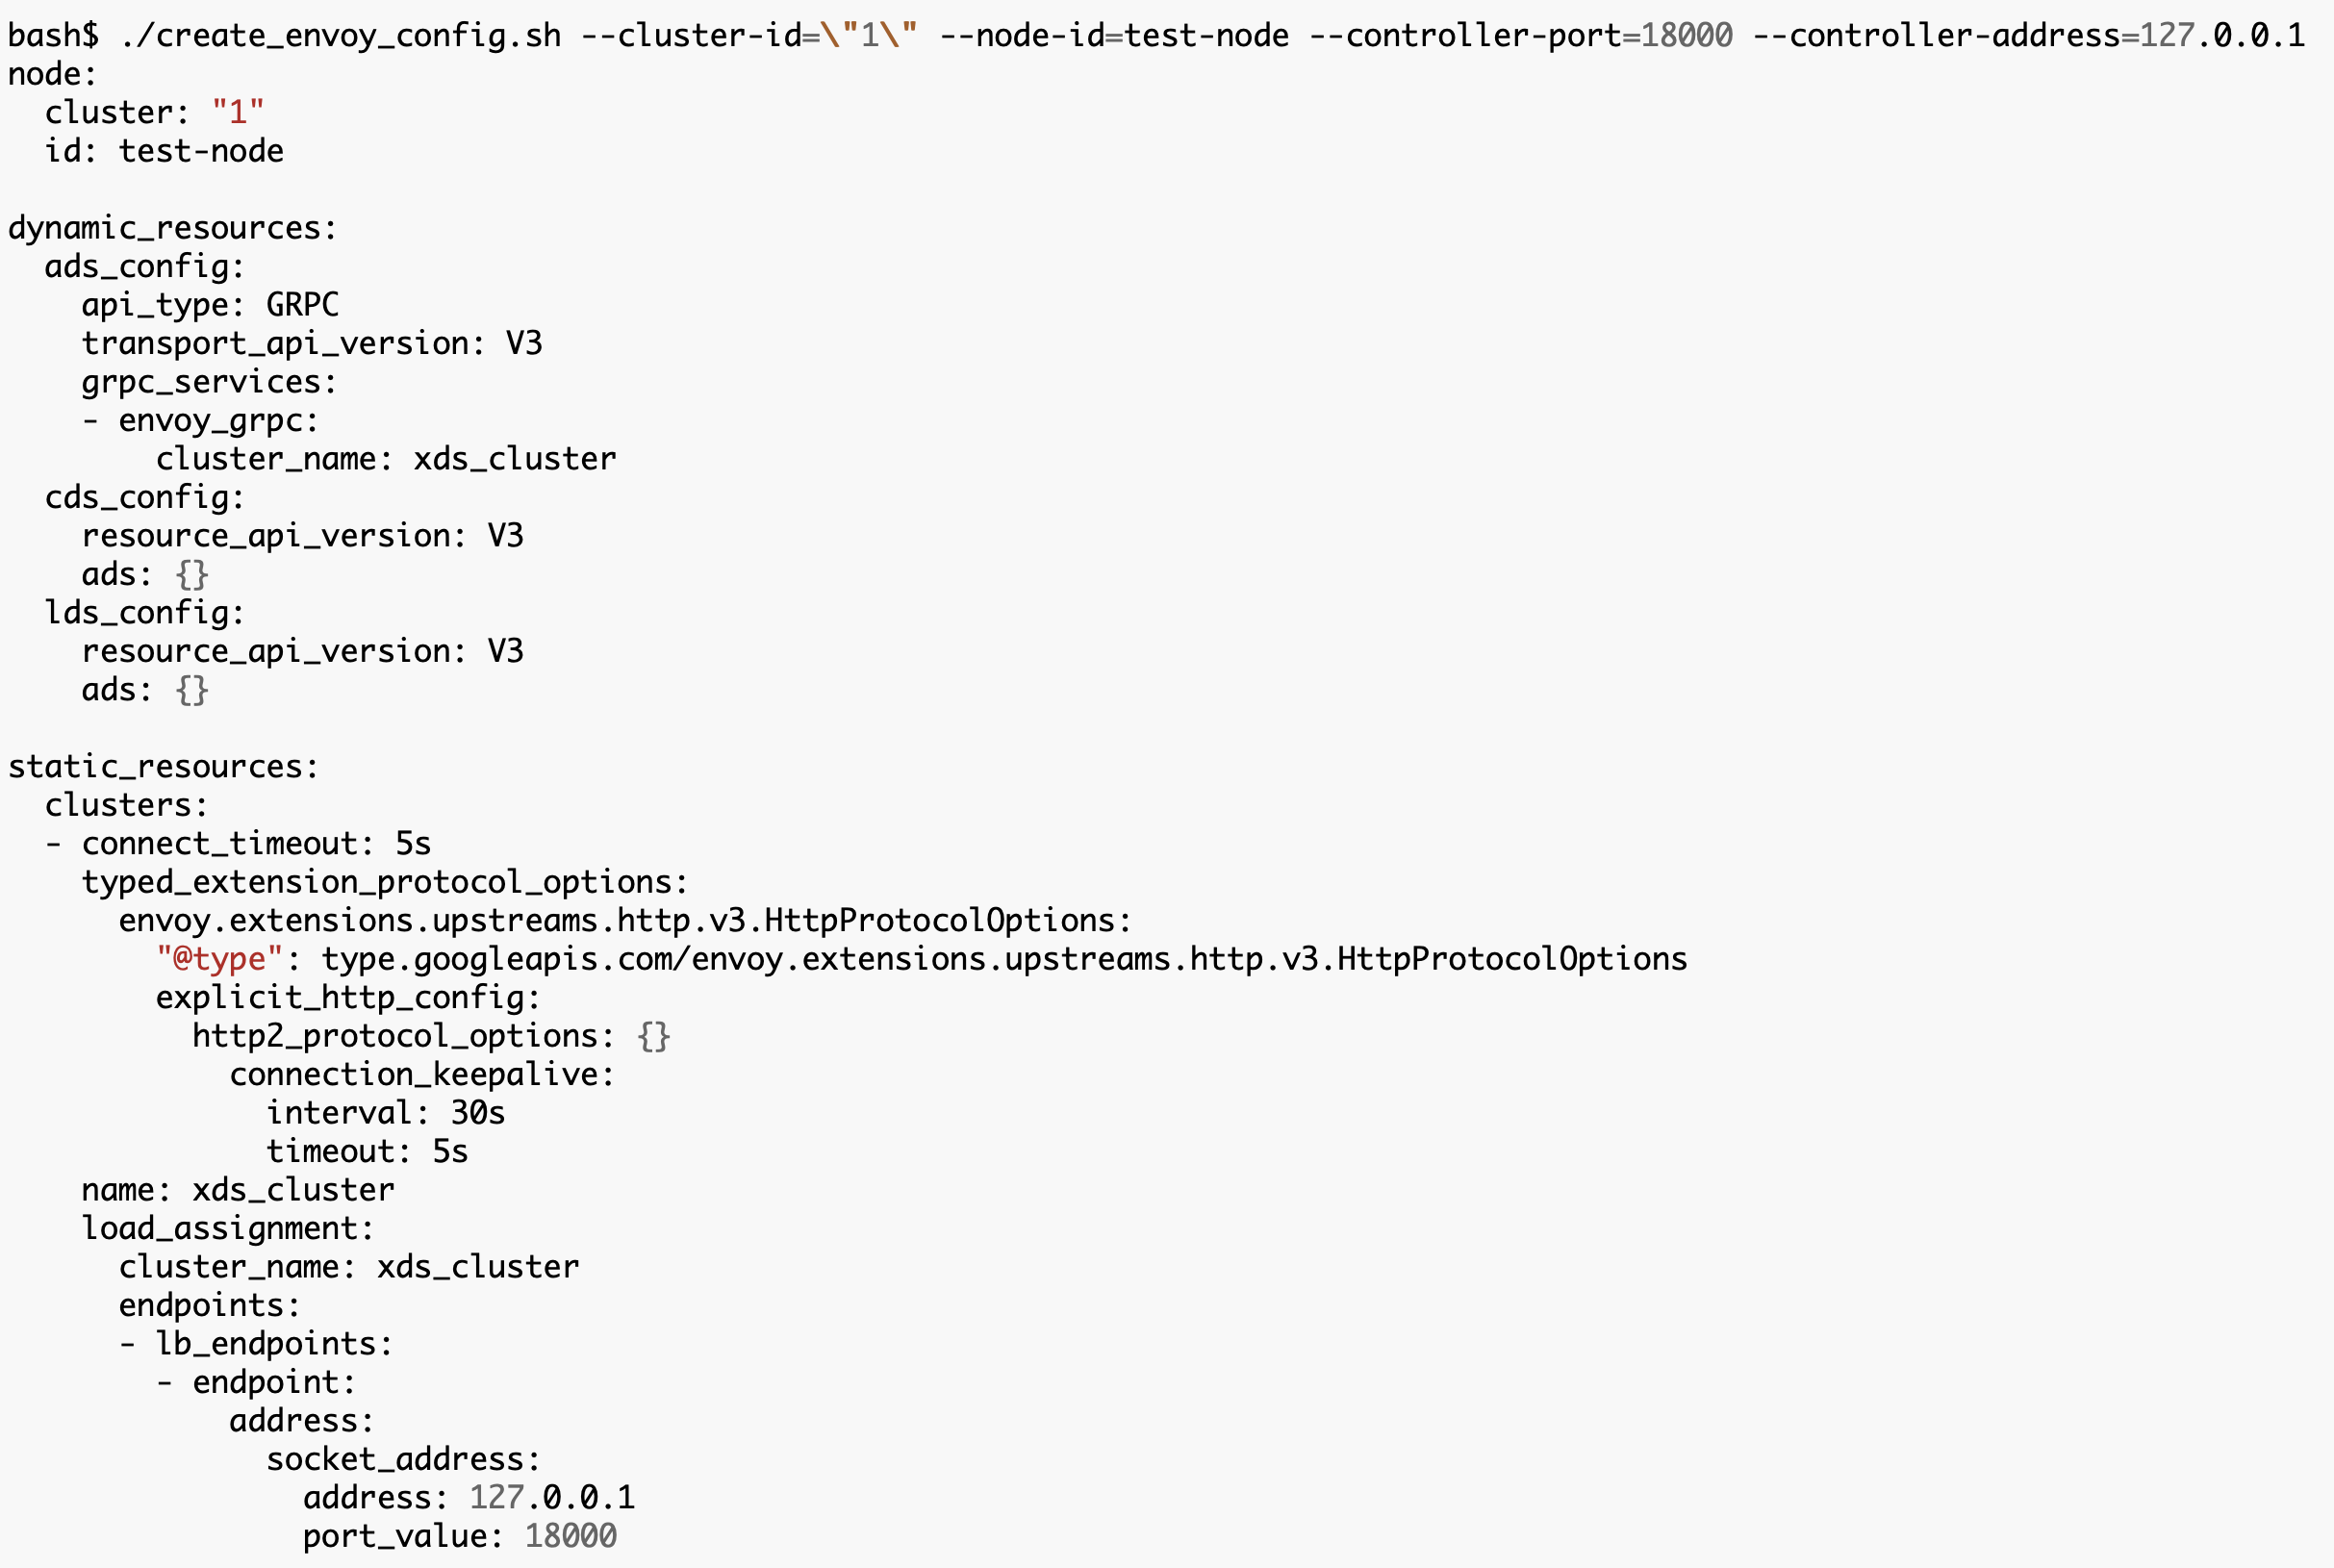
\includegraphics[width=\textwidth]{script.png}

\subsection{Протокол общения между Envoy и Controller}

Ранее было показано как происходит изначальная конфигурация Envoy и теперь можно перейти к тому, каким образом реализовано общение между Envoy и Controller. В качестве основы была взята библиотека java-control-plane \cite{EnvoyControlPlane}, где реализованы основные классы для создания control plane для Envoy и также приведена демонстрационная реализация, в которой все необходимые конфигурации Envoy лежат в HashMap. К сожалению, эта реализация нам не подходит. В нашей реализации Service Mesh есть компонента, ответственная за хранение информации о состояниях инстансов сервисов и которая умеет из этого знания определять, каким образом надо конфигурировать Envoy-proxy и также хранит у себя эти файлы. Конечно же, файлы, которые составляет Service Discovery сильно отличюется по формату от файлов, которые необходимы Envoy'y так как мы хотим инкапсулировать логику общения с Envoy в компоненту Controller, а в запросах к Controller'y мы хотим описывать в более простом формате требования к Envoy-proxy.

Сравнение запроса Service Discovery$\,\to\,$Controller и Controller$\,\to\,$Envoy.


Рассмотрим, как эта библиотека обрабатывает запросы Envoy'a на получение актуальной конфигурации, что происходит при создании нового gRPC-stream или при его рестарте и также на то, как происходит обновление конфигурации Envoy при изменении элементов в HashMap с конфигурациями Envoy в демонстрационной реализации.

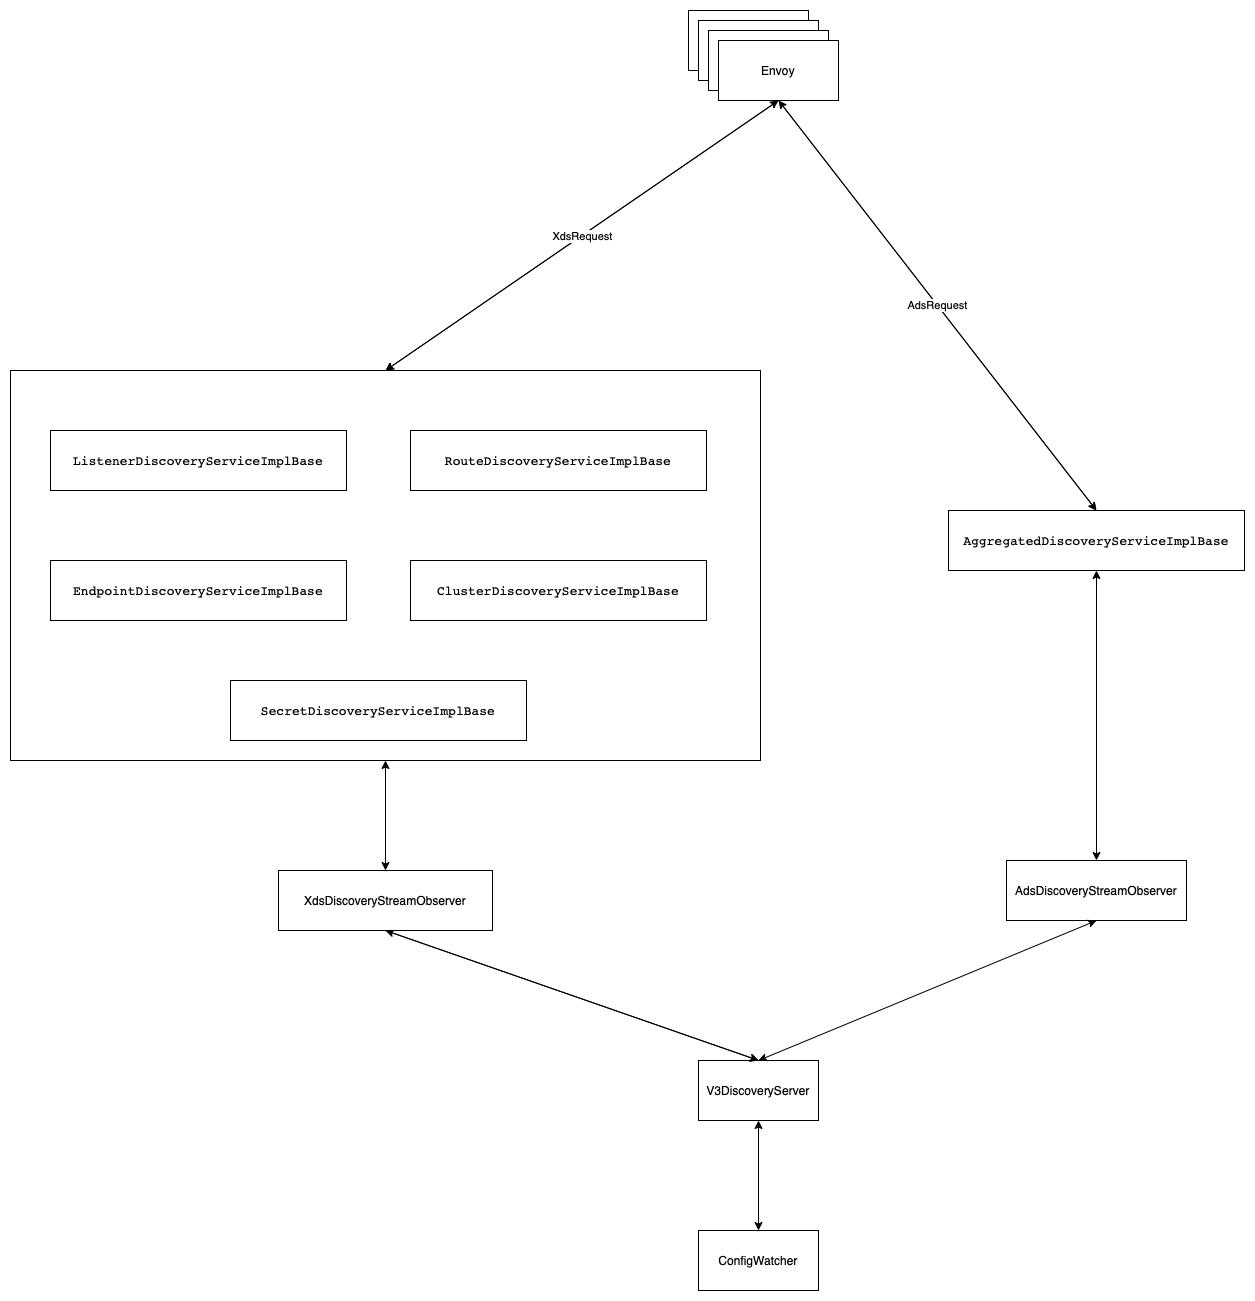
\includegraphics[width=\textwidth]{ControlPlaneArchitecture.png}

\begin{itemize}
    \item Envoy поддерживает двунаправленный gRPC-stream c несколькими gRPC сервисами из XDiscoveryServiceBase или с одним gRPC сервисом  AggregatedDiscoveryServiceImplBase. Я использую агрегированный gRPC-stream для всех типов ресурсов Envoy, поэтому это будет второй вариант.

    \item Далее запрос из gRPC-сервера обрабатывается с помощью XdsDiscoveryStreamObserver или с помощью AdsDiscoveryStreamObserver. В этой части происходит сведение обеих V2 и V3 типов запросов к единому интерфейсу и обогащения запроса информацией о последнем предыдущем запросе. 

    \item V3DiscoveryServer в этой цепочки выступает связывающим звеном. В нем храняться callback'и, которые следует вызывать при закрытии gRPC-stream'а и который передает запрос дальше в ConfigWatcher.

    \item ConfigWatcher выступает основной компонентой, которая следит за изменением конфигурации и до которой доходит вся предобработанная информация об исходном запросе. Именно здесь определяется, какую конфигурацию требуется отправить в Envoy. Для этих целей создается структура Watch, в которой хранится обработанный запрос от Envoy и функция, которую необходимо вызвать, чтобы получить требуемую конфигурацию.
\end{itemize}

Выше рассматривалась только ситуация, когда запрос поступает с Envoy, но мы также должны обрабатывать ситуации изменения конфигурации со стороны клиента, собственно, для этих целей и проектируется данное приложение. Для решения этой задачи достаточно в ConfigWatcher посмотреть на список всех зарегестрированных Watch'ей, найти среди них тот, который отвечает за необходимый нам тип ресурса Envoy, с помощью него отправить запрос  обновления конфигурации с помощью той же цепочки и удалить этот Watch так как после получения этого запроса Envoy обратно отправит сообщение о том, смог ли он перейти на новую версию.

Получается, что в этой цепочке надо сделать свою имплементацию ConfigWatcher, которая не будет внутри себя хранить HashMap, а будет следовать необходимой нам логике.
 
\subsection{Архитектура созданного приложения}
 
Рассмотрим, на какие компоненты делится приложение и как происходит обработка запроса на обновление конфигурации конкретного инстанса Envoy.

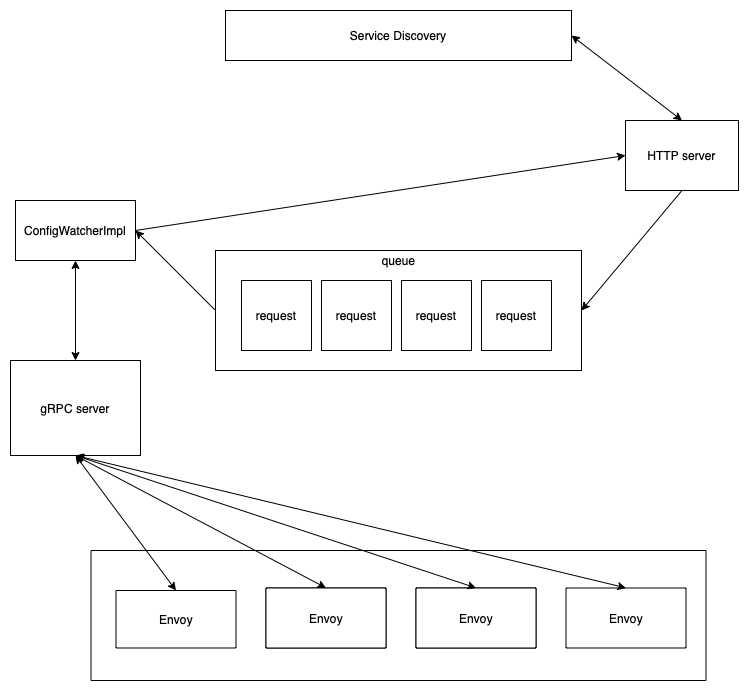
\includegraphics[width=\textwidth]{ControllerArchitecture.png}

\begin{itemize}
    \item Для начала нам нужен HTTP-server для прослушивания запросов, далее этот сервер может напрямую передовать эти запросы в ConfigWatcherImpl, но мы решили, что для Service Discovery было бы удобно, если запросы поступают батчами так как стоит учитывать что каждый из запросов выполняется не мгновенно, и также учитывая то, что иногда размер этого батча может равняться количеству инстансов некоторого сервиса, например, когда изменяются зависимости этого сервиса, а количество инстансов сервиса может быть достаточно велико, особенно в микросервисной архитектуре. Получается, что нам нужна очередь, чтобы складировать ресурсы, поэтому вместо передачи запросов в ConfigWatcherImpl он будет лежать в очереди.
    \item Далее возникает вопрос, что же использовать в качестве очереди. Здесь можно использовать или отдельное приложение для этого, например Kafka или RabbitMQ или пойти по более простому варианту и использовать встроянный в язык Java контейнер, такой как ArrayDeque. Я решил остановиться на последнем, так как сейчас нет предпосылок к тому, чтобы эта очередь не влезала в оперативную память и также у нас есть еще один ограниченный ресурс -- количество одновременно поддерживаемых gRPC-stream'ов и непонятно, какой из них заканчивается быстрее.
     \item У этой очереди будет обработчик, который по одному из сигналов 1) в пустую очередь добавился элемент; 2) 
 обработан предыдущий элемент и очередь не пустая; будет брать следующий элемент из очереди, трансформировать его в валидную Envoy-конфигурацию и перенаправлять в ConfigWatcherImpl. 
    \item ConfigWatcherImpl, как было описано в предыдущей части, через envoy-control-plane определяет, что необходимо послать в инстанс Envoy
    \item Через gRPC-server происходит передача сообщения Envoy и получение от него ответа.
    \item Ответ из gRPC-server'a передается в ConfigWatcherImpl, который его трансформирует в ответ для Service Discovery о том, что переконфигурирование произошло успешно или нет.
\end{itemize}

Также стоит показать, что происходит, когда запрос актуальной конфигурации приходит от самого Envoy. Это может произойти, например, при первичном создании gRPC-stream'a или когда этот gRPC-stream пересоздается. В данном случае обработка запроса происходит следующим образом.

\begin{itemize}
	\item gRPC-server принимает запрос, обрабатывает его, как было описано выше и передает в ConfigWatcherImpl
	\item ConfigWatcherImpl делает запрос к Service Discovery о получении необходимой конфигурации для инстанса Envoy с конкретным идентификатором ноды
	\item Через gRPC-server полученная конфигурация доставляется к инстансу Envoy и тот отвечает результатом переконфигурирования
	\item Результат переконфигурирования отправляется к Service Discovery
\end{itemize}
 
 \subsection{Тестирование}
 
 Заметим, что для тестирования нашего приложения нет необходимости создавать мини-систему, над которой работает Service Mesh, а достаточно просто запустить несколько приложений и для каждого из них динамически конфигурировать Envoy-proxy и смотреть, что они правильно работают. Также, к сожалению, не получится  просто отправлять Http-запросы к Controller, так как у него есть функционал, который отправляет запросы в Service Discovery, который тоже требуется протестировать. Получается, что необходимо проверить следующие функции приложения Controller:
 
 \begin{enumerate}
 	\item Можно конфигурировать Envoy как egress-proxy, то есть прокси, которая будет правильно обрабатывать запросы которые выходят из приложения и идут через прокси.
 	\item Можно конфигурировать Envoy как ingress-proxy, то есть прокси, которая получает запросы от других сервисов и должна перенаправить приложению
 	\item Корректность Http-запросов от Controller к Service Discovery.
 \end{enumerate}
 
 Для тестирования было написано приложение, эмулирующее Service Discovery следующим образом. Приложение Fake Service Discovery хранит в HashMap известные ему конфигурации Envoy и отдает их по запросу Controller. Также оно имеет Http-интерфейс, через который оно получает от пользователя новые конфигурации Envoy и запросы от Controller. Также было написано 2  приложения на Python, первое из которых является echo-server'ом, а второе выступает в роли Http-servera и в процессе работы использует этот echo-server.

 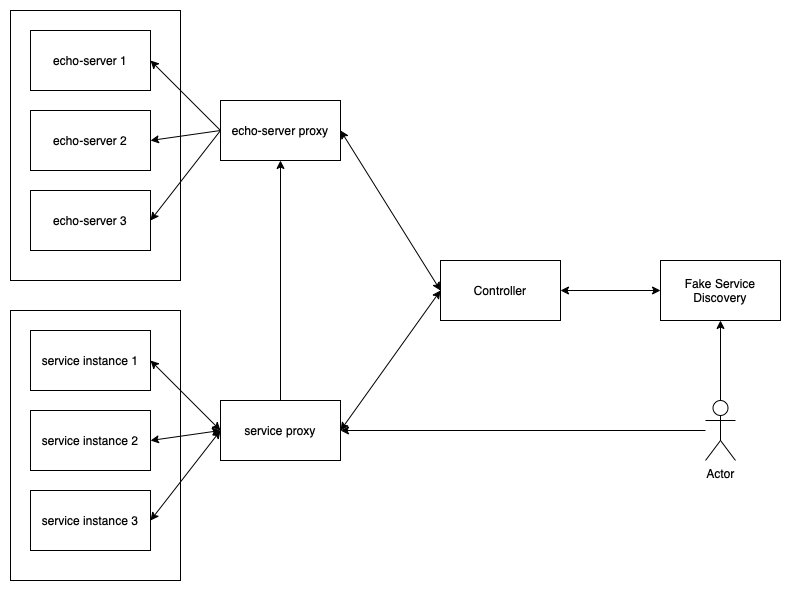
\includegraphics[width=\textwidth]{Test.png}

  Тестированаие проводилось следующим образом. Изначально было поднято 3 инстанса приложения service, 3 инстанса приложения ech-service и 2 Envoy proxy - по одному для каждого из них. Далее посылались запросы к service через его прокси, потом выбранный прокси инстанс сервиса отправлял запрос к echo-server, который изначально шел к service-proxy, который перенаправлял его к echo-service proxy и который, соответственно, перенаправлял его к нужному инстансу echo-server. Отправляя таким образом запросы проверялось, что прокси может выступать и как прокси на вход и как прокси на выход. Далее, через Fake Service Discovery посылались запросы на изменение колличества инстансов, о которых знают прокси и у echo-server и у service. Так проверялся протокол передачи сообщений между Controller и Service Discovery.    

\section{Результаты}

Приложения Controller и приложение для тестирования Fake Service Discovery были написаны на языке Java 17 с использованием фреймворка Spring и  библиотек io.envoyproxy.controlplane, io.grpc. Скрипт для создания шаблонной конфигурации Envoy был написан на языке bash. И приложения echo-server и service для тестирования были написаны на языке Python с использованием flask.

\section{Заключение}

В рамках данной работы проводилось исследование существующих подходов к реализации Service Mesh и на основе рассмотренных подходов была предложена архитектура Service Mesh для 1С облака. Также была реализовано приложение Controller, входящие в Service Mesh Control Plane и набор инструментов, позволяющих с легко настраивать Service Mesh Data Plane.

При дальнейших исследованиях планируется проверить колличество потребляемых ресурсов данного приложения при большей нагрузке и при негативных результатах можно рассматривать такие улучшения как смена транспортного протокола Envoy на то, чтобы в рамках запроса на обновление конфигурации не происходила полная переконфигурация, а только разница между текущей конфигурацией и новой. Также очередь запросов может переполниться и может потребоваться вынести ее в отдельное приложение, такое как Kafka или RabbitMQ.


Другим вектором для будущих исследований может быть добавление новой функциональности для Service Mesh, например, обеспечение безопсности.
%Имплементация описанного выше решения была написана на C++20 с использованием библиотек Eigen, Function2, GLFW3, Cxxopts и Vulkan. Исходный код имеет размер порядка 10000 строк и доступен по ссылке \url{https://github.com/Mrkol/thesis_vgi}.
%
%В качестве тестовых моделей были выбраны 3D-сканы Quixel Megascans \cite{quixel_megascans} в максимальном качестве. В следующей таблице приведено время работы этапов предобработки, а также количество полигонов и название использованных моделей. В столбец "подготовка" объединены этапы (1-2), в столбец "кластеризация" этапы (3-4), в "квадрангуляцию" -- (5-6), а последние 2 столбца соответствуют этапам (7) и (8). В разных строках указаны запуски с разной целевой ошибкой кластеризации, в столбце "кластеры" указано итоговое количество кластеров. Замеры происходили на Intel Core i5-470 (3.20Ghz) и видеокарте NVIDIA GeForce RTX 2070 SUPER.
%
%
%\begin{table}[ht]
%\small
%\centering
%\begin{tabular}{ l | p{16mm} | p{15mm} | p{17mm} | p{12mm} | p{14mm} | p{13mm} | p{17mm} }
%                        & Полигоны (млн.) & Кластеры & Подготовка (мин.) & Кластер. (мин.) & Квадранг. (мин.) & Репарам. (мин.) & Ресемплинг (мин.) \\
%\hline
%\multirow{2}{18mm}{Rock Cliffs (uchwaffda)}
%& 3    & 130 & 2.1   & 0.8  & 40   & 105    & 0.2   \\
%& 3    & 164 & 2.1   & 0.8  & 40   & 83     & 0.2   \\
%\hline
%\multirow{3}{16mm}{Rock Sandstone (rlbx3)}
%& 5    & 30  & 3.4   & 1.4  & 116  & 700    & 0.5   \\
%& 5    & 224 & 3.5   & 1.4  & 34   & 200    & 0.3   \\
%&&&&&&&\\
%\end{tabular}
%\caption{Производительность алгоритма предобработки}
%\end{table}
%
%Как видно из таблицы, время затраченное на репараметризацию сильно зависит от количества кластеров. Более того, при малом числе кластеров их форма как правило становится достаточно иррегулярной, что приводит к значительно большему времени на этапе квадрангуляции из-за необходимости делить рёбра. С другой стороны большее число кластеров приводит к более медленному рендерингу из-за необходимости адаптировать б\'ольшее число квадродеревьев.
%
%\begin{figure}[h]
%  \minipage{0.45\textwidth}
%    \begin{tikzpicture}
%      \begin{axis}[
%          scale=0.85,
%          ybar,
%          symbolic x coords={Минимум,Среднее,Максимум},
%          xtick=data,
%          enlarge x limits=0.2,
%          legend style={at={(0.025,0.975)}, anchor=north west},
%          ylabel={FPS}
%          ]
%        \addplot[ybar,fill=yellow] coordinates {
%          (Минимум,250) (Среднее,290) (Максимум,420)
%        };
%        \addplot[ybar,fill=red] coordinates {
%          (Минимум,200) (Среднее,260) (Максимум,682)
%        };
%        \addplot[ybar,fill=blue] coordinates {
%          (Минимум,24) (Среднее,26) (Максимум,457)
%        };
%        \legend{Уровни детализации,Предлагаемый метод,Исходная модель}
%      \end{axis}
%    \end{tikzpicture}
%    \caption{Производительность рендеринга модели ``Rock Cliffs (uchwaffda)'' в кадрах в секунду (FPS, frames per second). Больше -- лучше}
%    \label{fig:uchwaffda_perf}
%  \endminipage\hfill
%%
%  \minipage{0.45\textwidth}
%    \begin{tikzpicture}
%      \begin{axis}[
%          scale=0.85,
%          ybar,
%          symbolic x coords={Минимум,Среднее,Максимум},
%          xtick=data,
%          enlarge x limits=0.2,
%          legend style={at={(0.025,0.975)}, anchor=north west},
%          ylabel={FPS}
%          ]
%        \addplot[ybar,fill=yellow] coordinates {
%          (Минимум,130) (Среднее,140) (Максимум,250)
%        };
%        \addplot[ybar,fill=red] coordinates {
%          (Минимум,103) (Среднее,140) (Максимум,309)
%        };
%        \addplot[ybar,fill=blue] coordinates {
%          (Минимум,21) (Среднее,23) (Максимум,403)
%        };
%        \legend{Уровни детализации,Предлагаемый метод,Исходная модель}
%      \end{axis}
%    \end{tikzpicture}
%    \caption{Производительность рендеринга модели ``Rock Assembly Rough (sjzbj)'' в кадрах в секунду (FPS, frames per second). Больше -- лучше}
%    \label{fig:sjzbj_perf}
%  \endminipage\hfill
%\end{figure}
%
%Производительность и качество рендерига же измерялись на процессоре Intel Core i7-8550U и его встроенной видеокарте. Производительность алгоритма при движении камеры показана на рисунках \ref{fig:uchwaffda_perf}-\ref{fig:sjzbj_perf}. Для сравнения были взяты исходная высокополигональная модель отрендеренная и предоставляемые Quixel её уровни детализации. Из графиков видно, что использование иерархического атласа не сильно ухудшает производительность по сравнению с наивным использованием уровней детализации, но при этом в разы быстрее рендеринга полной исходной модели.
%
%Противопоставим эти показатели итоговому качеству картинки. Для его измерения была использована метрика SSIM \cite{wang2004image}, разработанная специально для сравнения видимого качества семантически одинаковых изображений. Сравниваемые изображения, а также изображения каркасов соответствующих моделей, представлены на рисунках \ref{fig:preview1start}-\ref{fig:preview3end}. Изображения полученные при помощи разработанного решения, а также полученные с помощью наивных уровней детализации, были сопоставлены с исходной высокополигональной моделью с трёх разных ракурсов. Результаты представлены на рисунке \ref{fig:quality}. Таким образом разработанное решение позволяет добиться качества на 20 процентных пунктов лучше наивного подхода, при этом незначительно проигрывая ему в производительности.
%
%\newcommand{\showpreviews}[1]{
%  \begin{figure}[h]
%    \minipage{0.32\textwidth}
%      \centering
%      \includegraphics[scale=0.079]{high#1}
%      \caption{Оригинальная модель. Вид с ракурса #1}
%      \label{fig:preview#1start}
%    \endminipage\hfill
%    \minipage{0.32\textwidth}
%      \centering
%      \includegraphics[scale=0.079]{ours#1}
%      \caption{Предлагаемый метод. Вид с ракурса #1}
%    \endminipage\hfill
%    \minipage{0.32\textwidth}
%      \centering
%      \includegraphics[scale=0.079]{lod#1}
%      \caption{Уровни детализации. Вид с ракурса #1}
%    \endminipage
%    \\
%    \minipage{0.32\textwidth}
%      \centering
%      \includegraphics[scale=0.079]{high#1_wireframe}
%      \caption{Оригинальная модель. Вид с ракурса #1 (сетка)}
%    \endminipage\hfill
%    \minipage{0.32\textwidth}
%      \centering
%      \includegraphics[scale=0.079]{ours#1_wireframe}
%      \caption{Предлагаемый метод. Вид с ракурса #1 (сетка)}
%    \endminipage\hfill
%    \minipage{0.32\textwidth}
%      \centering
%      \includegraphics[scale=0.079]{lod#1_wireframe}
%      \caption{Уровни детализации. Вид с ракурса #1 (сетка)}
%      \label{fig:preview#1end}
%    \endminipage
%  \end{figure}
%}
%
%\showpreviews{1}
%\showpreviews{2}
%\showpreviews{3}
%
%\begin{figure}[h]
%  \centering
%  \begin{tikzpicture}
%    \begin{axis}[
%        width=0.8\textwidth,
%        height=0.6\textwidth,
%        ybar,
%        ymin=0,ymax=1,
%        symbolic x coords={Разработанное решение,Уровни детализации},
%        xtick=data,
%        enlarge x limits=0.2,
%        ylabel={SSIM},
%        ]
%      \addplot[ybar,fill=yellow] coordinates {
%        (Разработанное решение,0.845) (Уровни детализации,0.627)
%      };
%      \addplot[ybar,fill=red] coordinates {
%        (Разработанное решение,0.844) (Уровни детализации,0.740)
%      };
%      \addplot[ybar,fill=blue] coordinates {
%        (Разработанное решение,0.834) (Уровни детализации, 0.640)
%      };
%    \end{axis}
%  \end{tikzpicture}
%  \caption{SSIM-качество отрендереных изображений с трёх ракурсов (обозначены цветами). Больше -- лучше}
%  \label{fig:quality}
%\end{figure}


%\section{Заключение}
%В рамках проведённой работы были уточнены детали устройства метода рендеринга с использованием иерархических атласов, предложен ряд усовершенствование в алгоритме отображения, а также разработано комплексное программное решение имплементирующее метод. Разработанное решение позволяет добиться значительного прироста в качестве картинки по сравнению с наиболее распространённым методом, уровнями детализации. Производительность решения удовлетворительна на этапе предобработки и сравнима с наивным подходом на этапе рендеринга.
%
%В силу большой модульности и сложности метода предобработки, при дальнейших исследованиях планируется повышать производительность и качество практически всех его частей. Планируется реализовать некоторое количество альтернативных подходов и сравнить получаемое качество, а также время предобработки. Среди прочего планируются исследования в направлении поддержки неоднородных вершинных атрибутов посредством проведения границ кластеров по границам разрывов, ускорение этапа репараметризации используя иные алгоритмы оптимизации, использование иных методов кластеризации, а также внедрение модификаций предлагаемых в \cite{feng2010feature}. Планируется пересмотр этапа распрямления границ. В результате этой операции эвристика планарности кластеров сильно ухудшается, что в некоторых ситуациях приводит к недостаточной частоте семплирования выступов моделей. Более тонкий учёт геометрии поверхности на этапе сглаживания может помочь избавится от этой проблемы. Отметим, что аналогичный эффект проявляется и на этапе квадрангуляции, но в меньшей степени.
%
%Ещё одним крупным направлением для дальнейших исследований являются алгоритмы адаптации при рендеринге иерархического атласа. Также планируется внедрение параллелизма в текущую имплементацию рендеринга (вынесение обновления виртуального кэша в отдельный поток), и наконец рассмотрение возможности перенесения вычислений нагружающих центральный процессор в текущей имплементации (адаптация, вычисление мип уровней для границ) на графический процессор.
%
%По мнению автора подход виртуализации весьма перспективен в применении к современным приложениям реального времени, так как способен удовлетворить всё растущие требования к визуальному качеству, а также позволяет более эффективно использовать ресурсы GPU, а поэтому заслуживает дальнейшего изучения и усовершенствования.


\newpage
\printbibliography[title=Источники]
\end{document}